%% Copyright 2018 H.\ Rabus
%
% This work may be distributed and/or modified under the
% conditions of the LaTeX Project Public License, either version 1.3
% of this license or (at your option) any later version.
% The latest version of this license is in
%   http://www.latex-project.org/lppl.txt
% and version 1.3 or later is part of all distributions of LaTeX
% version 2005/12/01 or later.
%
% This work has the LPPL maintenance status `author-maintained'.
%
% This work consists of the file texbsp.tex
%

\documentclass[smallheadings]{scrartcl}

%%% GENERAL PACKAGES %%%%%%%%%%%%%%%%%%%%%%%%%%%%%%%%%%%%%%%%%%%%%%%%%%%%%%%%%%
% inputenc allows the usage of non-ascii characters in the LaTeX source code
\usepackage[utf8]{inputenc}
\usepackage{graphicx} 
\graphicspath{ {/u/hnatiuka/Praktikum/PPI/} }



% title of the document
\title{Dokumentation Serie 1 -- Teil 1}
% optional subtitle
%\subtitle{Draft from~\today}
% information about the author
\author{%
  Arsen Hnatiuk,\\%
  Max Huneshagen 
}
\date{\today} 


%%% LANGUAGE %%%%%%%%%%%%%%%%%%%%%%%%%%%%%%%%%%%%%%%%%%%%%%%%%%%%%%%%%%%%%%%%%%
% babel provides hyphenation patterns and translations of keywords like 'table
% of contents'
\usepackage[ngerman]{babel}

%%% HYPERLINKS %%%%%%%%%%%%%%%%%%%%%%%%%%%%%%%%%%%%%%%%%%%%%%%%%%%%%%%%%%%%%%%%
% automatic generation of hyperlinks for references and URIs
\usepackage{hyperref}

%%% MATH %%%%%%%%%%%%%%%%%%%%%%%%%%%%%%%%%%%%%%%%%%%%%%%%%%%%%%%%%%%%%%%%%%%%%%
% amsmath provides commands for type-setting mathematical formulas
\usepackage{amsmath}
% amssymb provides additional symbols
\usepackage{amssymb}
% HINT
% Use http://detexify.kirelabs.org/classify.html to find unknown symbols!

%%% COLORS %%%%%%%%%%%%%%%%%%%%%%%%%%%%%%%%%%%%%%%%%%%%%%%%%%%%%%%%%%%%%%%%%%%%
% define own colors and use colored text
\usepackage[pdftex,svgnames,hyperref]{xcolor}

%%% Code Listings %%%%%%%%%%%%%%%%
% provides commands for including code (python, latex, ...)
\usepackage{listings}
\definecolor{keywords}{RGB}{255,0,90}
\definecolor{comments}{RGB}{0,0,113}
\definecolor{red}{RGB}{160,0,0}
\definecolor{green}{RGB}{0,150,0}
\lstset{language=Python, 
        basicstyle=\ttfamily\small, 
        keywordstyle=\color{keywords},
        commentstyle=\color{comments},
        stringstyle=\color{red},
        showstringspaces=false,
        identifierstyle=\color{green},
        }


\usepackage{paralist}

% setting the font style for input und returns in description items
\newcommand{\initem}[2]{\item[\hspace{0.5em} {\normalfont\ttfamily{#1}} {\normalfont\itshape{(#2)}}]}
\newcommand{\outitem}[1]{\item[\hspace{0.5em} \normalfont\itshape{(#1)}]}
\newcommand{\bfpara}[1]{
	
	\noindent \textbf{#1:}\,}

\begin{document}

% generating the title page
\maketitle
% generating the table of contents (requires to run pdflatex twice!)
\tableofcontents
\bigskip

\hrule
\hrule

%%% BEGIN OF CONTENT %%%%%%%%%%%%%%%%%%%%%%%%%%%%%%%%%%%%%%%%%%%%%%%%%%%%%%%%%%

\section{Einleitung}

Aus der Theorie der Taylorentwicklung kann man ein günstiges Verfahren zur Approximation der ersten und zweiten Ableitungen einer Funktion ableiten. Dieses Verfahren nennt man die Methode der Vorwärtsdifferenz. Dieses Programm erlaubt eine numerische Analyse dieses Verfahrens. Insbesondere dient dieses Programm zur Berechnung des absoluten Fehlers dieses Verfahrens und zur Veranschaulichung der Beziehung zwischen diesem Fehler und anderen Parametern. 

\section{Schnittstellendokumentation \emph{plotten.py}}

Diese Klasse erlaubt das Plotten von Funktionen und ihren Ableitungen. Die Ableitungen werden dabei approximiert oder können als exakte Funktionen übergeben werden. 

\subsection{Attribute}

\textbf{nicht-statische Attribute:}\\

\begin{compactdesc}
	\initem{plotbereich}{pyplot.Axes-Objekt} The operating system, that is currently run on the computer.
                      Should be one of the values `MAC`, `WINDOWS` or `LINUX`
	      \initem{unten}{float} Untere Intervallgrenze.
	      \initem{oben}{float} ~\\ Obere Intervallgrenze.
\end{compactdesc}



%%%%%%%%%%%%%%%%%%%%%%%%%%%%%%%%%%%%%%%%%%%%%%%%%%%%%%%%%%%
%%%%%%%%%%%%%%%%%%%  Beginn Arsens Teil

\section{Bedienungsanleitung zum Hauptprogramm}

In der Datei \texttt{hauptprogramm.py} wird eine \texttt{main()} Methode implementiert. In dieser Methode werden alle Objekte erstellt, die später zur graphischen Darstellung des Fehlerplots dienen. Es werden auch die in der \texttt{differenzieren} Klasse definierten Methoden mittels der Beispielfunktion (Sinus) veranschaulicht. 

Zuerst wird der Benutzer gefordert, eine Schrittweite einzugeben. Es muss eine beliebige nichtnegative \texttt{float} Zahl eingegeben werden. Die Gültigkeit des Eingabetyps wird durch \texttt{exceptions} behandelt, und danach durch eine \texttt{if} Schleife auf Positivität geprüft. Eine nicht gültige Eingabe wird nicht berücksichtigt  und der Benutzer wird erneut gefordert, eine Eingabe zu machen.

Diese Kontrolle erfolgt auf die folgende Weise:

\begin{lstlisting}
abbr = 1 
while abbr == 1: 
    try:
        h_test = float(input('Mit welcher Schrittweite wollen Sie die' + 
        ' Ableitungen  approximieren?\n' +
        'Schreiben Sie bitte eine echt positive Zahl, z.B. 0.1\n'))
        abbr = 0
    except ValueError:
        print('Nicht gueltiger Wert eingegeben. Versuchen Sie erneut.')
        abbr = 1
    if h_test <= 0:
        print('Nicht gueltiger Wert eingegeben. Versuchen Sie erneut.')
        abbr = 1
\end{lstlisting}

Danach wird die Beispielfunktion (die Sinus Funktion) bearbeitet. Es werden Die \texttt{subplots} und die \texttt{arrays} erzeugt, auf welchen die Abbildungen geplottet und entsprechend evaluiert und approximiert werden. Ein Objekt der \texttt{differenzieren} Klasse für die Sinus Abbildung wird auch erzeugt.  Schließlich wird die Sinus Abbildung samt seinen zwei ersten Ableitungen
und der Approximation (für die durch den Benutzer eingegebene Schrittweite) dieser Ableitungen mittels der in der \texttt{differenzieren} Klasse definierten Methoden graphisch dargestellt. Der absolute Fehler der Approximation jeder von den zwei Ableitungen wird dann im Terminal ausgedruckt. 

Anschließend wird die Funktion \texttt{fehlerplot()} aufgerufen, um die Beziehung zwischen dem absoluten Fehler und der Schrittweite zu veranschaulichen. 

\subsection{fehlerplot()}

In dieser Funktion wird ein Plot des absoluten Fehlers in Abhängigkeit von der Schrittweite mittels der Differenzieren Klasse gezeichnet. Diese Funktion benutzt insbesondere die \texttt{np.vectorize} Methode, um Arrays mit den Fehlerwerten zu erzeugen, und die \texttt{.loglog} Methode, um eine doppelt-logarithmisch skalierte Graphik zu erstellen.

\paragraph{Input}
\begin{compactdesc}
	\initem{plotbereich}{pyplot.Axes-Objekt} Subplot, auf dem das Plot erzeugt wird
	\initem{diff\_objct}{Differenzieren-Instanz} Differenzieren-Obejekt, das untersucht wird
	\initem{h\_array}{numpy.ndarray aus floats} Array mit den Schrittweiten
\end{compactdesc}

\paragraph{Output}

Diese Funktion hat keinen Output

\subsection{Beispieldurchlauf}

Hier is ein Beispieldurchlauf. Der eingegebene Wert für die Schrittweite ist \texttt{0.1}.

\begin{verbatim}
Mit welcher Schrittweite wollen Sie die Ableitungen approximieren?
Schreiben Sie bitte eine echt positive Zahl, z.B. 0.1
0.1
Der absolute Fehler in der ersten Ableitung ist 0.04999, Schrittweite 0.10
Der absolute Fehler in der zweiten Ableitung ist 0.00083, Schrittweite 0.10
\end{verbatim}

Es werden dazu zwei Graphiken erzeugt (Abbildung 1). Man sieht auf der linken Seite eine Graphik mit dem absoluten Fehler als Funktion von der Schrittweite. Auf der rechten Graphik steht die Beispielfunktion mit ihren Ableitungen (exakt und approximiert).

\begin{figure}
	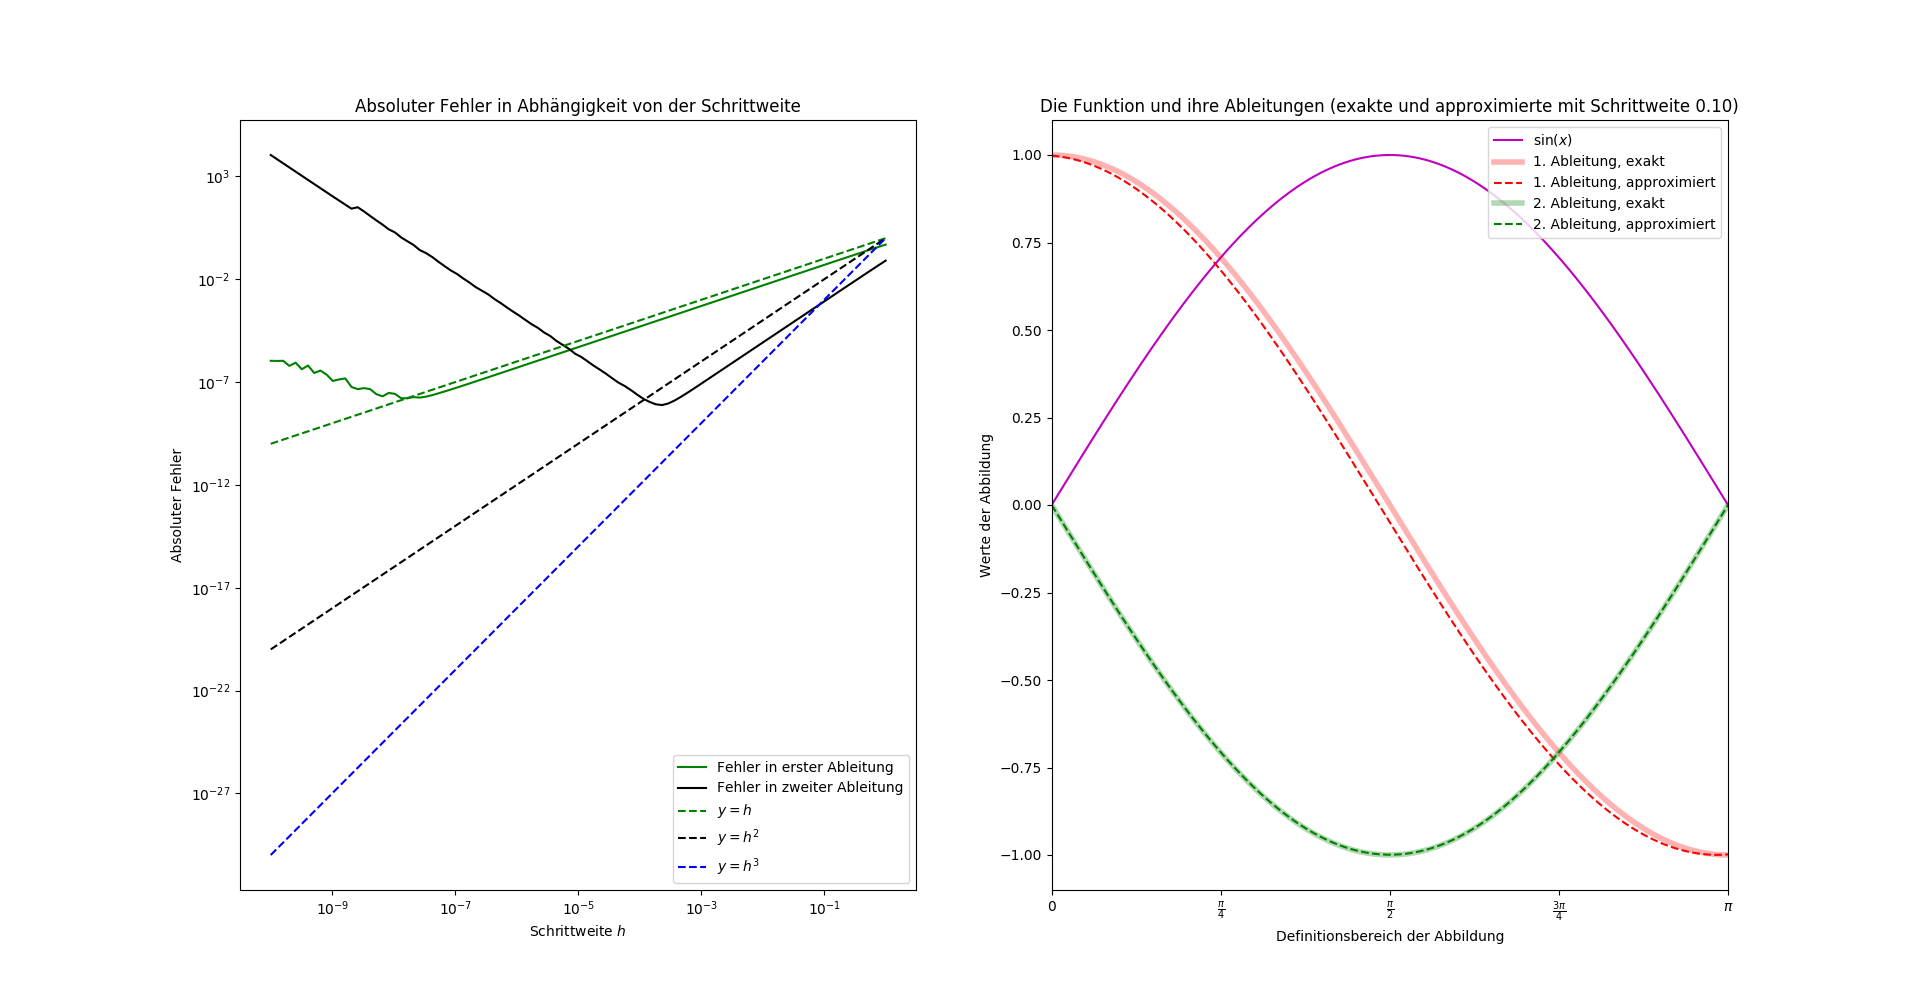
\includegraphics[width=\linewidth]{Figure_1.png}
	\caption{Die ausgegebene Graphik}
	\label{Abbildung 1}
\end{figure}

%%% END OF DOCUMENT %%%%%%%%%%%%%%%%%%%%%%%%%%%%%%%%%%%%%%%%%%%%%%%%%%%%%%%%%%%
\end{document}
